\documentclass{apuntes}

\usepackage{tikztools}

\title{HistoriaMatematicas}
\author{Pedro Valero}
\date{15/16 C1}

% Paquetes adicionales

% --------------------

\begin{document}
\setcounter{tocdepth}{4}

\pagestyle{plain}
\maketitle

\begin{abstract}
Este documento resume de modo esquemático las ideas vistas en la asignatura de Historia de las Matemáticas. Desde el punto de vista matemático, este resumen pretende ser completo aunque no desde el punto de vista histórico.

Aunque se realizarán algunas menciones a determinados detalles contextuales, se recomienda encarecidamente la lectura de los apuntes proporcionados por el profesor para una mejor comprensión del contenido histórico de la asignatura.
\end{abstract}

\tableofcontents
\newpage
% Contenido.

\chapter{La antigua Grecia}

\section{Pitágoras}
El teorema de Pitágoras, bien conocido por todos, llamó enormemente la atención de los griegos desde el momento de su descubrimiento.

Una vez planteada la identidad que reza el teorema hay dos cosas fundamentales que hacer a continuación:
\begin{enumerate}
\item Demostrar el enunciado del Teorema
\item Generar triángulos rectángulos que satisfagan el Teorema \textbf{con longitudes enteras}
\end{enumerate}


\begin{defn}[Ternas Pitagóricas]
Dada una tupla de tres números enteros $(a,b,c)$, diremos que es una \textbf{terna pitagórica}, es decir, $(a,b,c) \in \algb{T}$ si satisface:
\[a^2+b^2=c^2\]
\end{defn}

\subsection{Generación de ternas pitagóricas}
\subsubsection{Teorema de Euclides y Diofanto}
Para calcularlas podemos emplear el Teorema de Euclides y Diofanto que veremos a continuación:
\begin{theorem}[Teorema de Euclides y Diofanto (300-250 a.c.)]
Dada una terna $(a,b,c)$,
\[(a,b,c) \in \algb{T} \iff \left\{ \begin{array}{l} a = (p^2-q^2)\cdot r \\ b = 2\cdot p\cdot q\cdot r \\ c = (p^2+q^2)\cdot r\end{array}\right.\]

para algunos valores de $p,q,r \in \nat$.
\end{theorem}

\begin{proof}
Demostrar la implicación de derecha a izquierda es trivial, basta con operar.

Veamos cómo hicieron los griegos la demostración de la existencia de los $p,q,r$ que aparecen en el teorema. La demostración se basa en ir dando pequeños pasos que nos permiten acercarnos poco a poco al resultado deseado:

\begin{enumerate}
\item \textbf{Ternas primitivas}

Sea $k=m.c.d.(a,b,c)$, podemos escribir:
\[\begin{array}{l} a=ka' \\ b=kb' \\ c=kc' \end{array}  \implies K^2(a'^2+b'^2)=a^2+b^2 = c^2=k^2c'^2 \implies c'^2=a'^2+b'^2\]

Es decir, que podemos dividir todos los elementos de la terna entre $k$ y obtendríamos una nueva terna con la que trabajar. 

Por tanto, vamos a considerar sin pérdida de generalidad que $m.c.d.(a,b,c) = 1$. A las ternas que satisfagan esta condición las llamaremos \textbf{ternas primitivas}.

\item \textbf{Los elementos de una terna primitiva son coprimos dos a dos}

Vamos a demostrar, por reducción al absurdo que $(a,b,c) \in \algb{T} \y m.c.d.(a,b,c)=1 \implies m.c.d(a,b)=1$.
\begin{proof}
Sea $k=m.c.d.(a,b)$, podemos escribir:
\[\begin{array}{l} a=ka' \\ b=kb' \\ c=a^2+b^2 \implies k^2(a'^2+b'^2) \implies m.c.d.(a,b,c)=k \neq 1 \end{array}\]
\end{proof}

De forma equivalente podemos demostrar que dos elementos cualesquiera de una terna pitagórica primitiva son coprimos.

\item \textbf{Paridad de los elementos de la terna}

Sabiendo que se tiene que satisfacer la relación $a^2+b^2=c^2$ vamos a estudiar las diferentes posibilidades:

\begin{itemize}
\item \textbf{a,b pares}

Este caso no puede darse puesto que han de ser coprimos.

\item \textbf{a,b impares}

En este caso tendríamos:
\[a^2+b^2 \text{ par } \implies c^2 \text{ par } \implies c \text{ par}\]

Así tendríamos:
\[\begin{array}{l} a=2m+1 \\ b = 2n+1 \\ c^2 =(2m+1)^2+(2n+1)^2 = 4(n^2+m^2+n+m)+2\end{array} \]

y, puesto que $c$ es par, sabemos que $\frac{c^2}{2}$ también lo será, pero:
\[\frac{c^2}{2} = 2(n^2+m^2+n+m)+1 \text{, que es impar con lo que tendríamos una contradicción}\]

\item \textbf{a impar, b par}

En este caso tendríamos
\[a^2+b^2 \text{ impar } \implies c^2 \text{ impar } \implies c \text{ impar}\]

Podemos ver ahora que las fracciones 
\[\frac{c-a}{b}=\frac{p}{q} \text{ y } \frac{c+a}{b}=\frac{q}{p} \text{ no son irreducibles}\]

\obs Para ver que una fracción es la inversa de la otra (como se intuye al escribirlas como $p/q$ y $q/p$ respectivamente) basta con igualar una con la inversa de la otra y ver que el Teorema de Pitágoras garantiza la igualdad.

Si ahora sumamos y restamos ambas fracciones tenemos:
\[\frac{2c}{b}=\frac{p}{q}+\frac{q}{p} \iff \frac{c}{b}=\frac{p^2+q^2}{2pq}\]
\[\frac{2a}{b}=\frac{p}{q}-\frac{q}{p} \iff \frac{a}{b}=\frac{p^2-q^2}{2pq}\]

De aquí podemos deducir:
\[\left\{ \begin{array}{l} a=p^2-q^2 \\ b=2pq \\ c=p^2-q^2 \end{array} \right.\]

\end{itemize}
Y ya tenemos el resultado buscado, salvo por un detalle, el factor $r$. 

Ahora sólo tenemos que volver la vista al inicio de la demostración y comprobar que estábamos considerando ternas primitivas, para lo que sacamos factor común. Este factor común será la $r$ que necesitamos.
\end{enumerate}
\end{proof}

\subsubsection{Relación entre las ternas pitagóricas y cicunferencia unidad}

La idea se apya e que dado un punto de la circunferencia unidad, la ecuación que lo describe, $x^2+y^2=1$ se asemeja a otra que podemos obtener a partir del Teorema de Pitágoras:
\[a^2+b^2=c^2 \implies \left(\frac{a}{c}\right)^2 + \left(\frac{b}{c} \right)^2 = c^2\]

Por lo que parece razonable pensar que cada coordenada racional de la circunferencia unidad está asociada a una terna pitagórica. Así llegaron al siguiente teorema

\begin{theorem}
$(a,b,c)\in \algb{T} \iff \left( \frac{a}{c},\frac{b}{c}\right)$ es coordenada racional de la circunferencia unidad. 
\end{theorem}
\begin{proof}
La demostración de izquierda a derecha es trivial y se consigue simplemente haciendo cuentas.

Vamos hacer la demostración de derecha a izquierda.

Sea $(x,y)$ una coordenada racional de la circunferencia unidad, podemos escribirla como $(\frac{p}{q},\frac{r}{s})$ y sabemos que
\[\left( \frac{p}{q}\right)^2 + \left( \frac{r}{s}\right)^2 = 1 \iff (sp)^2+(qr)^2=(qs)^2\]
con lo que ya hemos obtenido una terna pitagórica: $(sp,qr,qs)\in \algb{T}$ 
\end{proof}

\subsubsection{Obtención de ternas pitagóricas a partir de la circunferencia unidad}

Ya hemos visto que todas las coordenadas racionales de la circunferencia unidad dan lugar a una terna pitagórica. La idea ahora es ver cómo podemos encontrar estas coordenadas racionales.

La idea es muy sencilla. Si tomo rectas que salgan del $(-1,0)$ con pendientes racionales, al intersecas estas rectas con la circunferencia, obtendremos coordenadas raciones.

La demostración es trivial y sólo requiere construir la recta con pendiente $\frac{p}{q}$ y comprobar que, efectivamente la intersección es un punto racional.

Se deja como ejercicio para el lector.

También es muy sencillo de comprobar que el recíproco es cierto, basándonos en la definición de la pendiente. Si tenemos dos puntos racionales en el plano, la pendiente será un número racional puesto que no hacemos más que restarl y dividir las coordenadas racionales.


\subsection{Demostraciones del Teorema de Pitágoras}
Los griegos mostraron tal fascinación por el Teorema de Pitágoras que idearon numerosas demostraciones del mismo. A continuación veremos algunas de ellas.

\subsubsection{Prueba 1}
Partiendo del siguiente diagrama:
\begin{center}
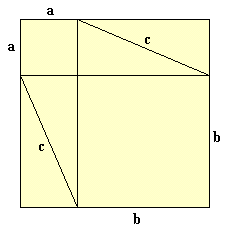
\includegraphics[width=0.8\linewidth/2]{img/pitagoras1.png}
\end{center}

Podemos comprobar sencillamente que el area del cuadrado menor es igual a la suma de las áreas de los triángulos y del cuadrado menor. 

Así tenemos:
\[(a+b)^2 = c^2 + \frac{ab}{2}\cdot 4 \iff a^2+b^2 +2ab = c^2 +2ab \iff a^2+b^2=c^2\]

\subsubsection{Prueba 2}
Partiendo del siguiente diagrama:
\begin{center}
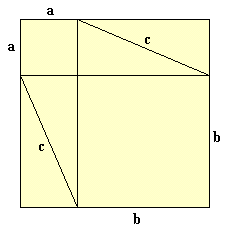
\includegraphics[width=0.8\linewidth/2]{img/pitagoras1.png}
\end{center}

Podemos encontrar de nuevo una relación entre las áreas de los cuadrados y triángulos pintados:
\[a^2+b^2 +4\frac{ab}{2} = (a+b)^2 \iff a^2+b^2 +2ab = a^2+b^2+2ab \iff a^2+b^2=c^2\]

\subsubsection{Prueba 3 (Euclides)}
Partiendo del siguiente diagrama:
\begin{center}
\inputtikz{pitagoras_prueba_3}
\end{center}

Podemos observar que las dos líneas son azules, por triangulación.

TO BE CONTINUED...


\subsection{Las distancias}
A raíz del Teorema de Pitágoras, el ejemplo tan trivial que supone un triángulo rectángulo con los dos catetos de longitud $1$ nos lleva a la aparición de nuevos números que no son racionales y que, ante la visión del mundo de los griegos, no son números.

Los griegos consideraban que todos los números eran racionales por lo que, al toparse con lo que hoy en día conocemos como irracionales (como es el caso de $\sqrt{2}$) decidieron denominarlo distancia o magnitud.

Así, los irracionales tenían un sentido geométrico pero no eran considerados como números.

\subsubsection{Demostración de la irracionalidad de $\sqrt{2}$}

La demostración puede hacerse por reducción al absurdo.

Supongamos que es racional, entonces existen $p,q \in \ent$, coprimos entre si, tales que:
\[\sqrt{2} = \frac{p}{q} \implies p^2=2q^2 \implies p^2 \text{ par } \implies p \text{ par } \implies p=2s \text{ con } s \in \nat\]

Así tenemos:
\[(2s)^2 = 2q^2 \implies 2s^2 = q^2 \implies q^2 \text{ par } \implies q \text{ par}\]

con lo que tenemos una contradicción, pues considerábamos que $p$ y $q$ eran coprimos por lo que no pueden ser pares.

\section{Tales de Mileto}
Tales de Mileto era un filósofo que se planteó qué era la naturaleza y dejó tras de si una escuela formada por sucesores como Anaxágoras y Anaximandro, que se dedicaron a la especulación física.

Son numerosos los teoremas y proposiciones que se le atribuyen a tales, veamos algunos de ellos:
\begin{theorem}[Teoremas de Tales]
Los enunciados que se muestran a continuación dependen de los siguientes dibujos:

\begin{minipage}{0.57\textwidth}
\begin{center}
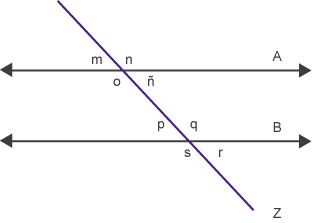
\includegraphics[width=\linewidth/2]{img/tales1.png}
\end{center}
\end{minipage}
\begin{minipage}{0.40\textwidth}
\begin{center}
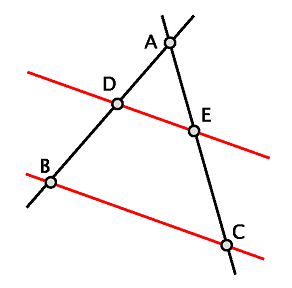
\includegraphics[width=\linewidth/2]{img/tales2.png}
\end{center}
\end{minipage}

\begin{enumerate}
\item Dadas dos rectas paralelas cortadas por una secante (ver figura de la izquierda) siempre se cumple:
\[m=p, \;\; n=q, \;\; o=s, \;\; \tilde{n}=r\]

\item Los ángulos opuestos por el vértice son iguales. Es decir:
\[m=\tilde{n}, \;\; n=o\]

\item La suma de los ángulos de un triángulo es π

\obs Esta afirmación puede demostrarse a partir de las dos anteriores

\item Todo diámetro divide a la circunferencia en dos partes iguales

\item Dos lados/ángulos iguales en un triángulos implican dos ángulos/lados iguales repectivamente.

\item \textbf{Semejanza}. Si tenemos dos triángulos proporcionales, como se muestra en la figura de la derecha, se cumple que:
\[\frac{\overline{AD}}{\overline{AB}} = \frac{\overline{AE}}{\overline{AC}} =\frac{\overline{DE}}{\overline{BC}}\]
\end{enumerate}
\end{theorem}


\subsection{Area del triángulo}
Es bien conocido por todos que la fórmula para el área del triángulo dice:
\[A= \frac{\text{base}\cdot\text{altura}}{2}\]
lo importante son las diferentes demostraciones existentes de esta fórmula, que veremos a lo largo de esta sección.

\begin{lemma}
El área de un triángulo rectángulo es proporcional al lado y la constante depende del ángulo
\end{lemma}
\begin{proof}
Dado el siguiente dibujo
\begin{center}
\inputtikz{thales_triangulo}
\end{center}
Sabemos, por el \textbf{teorema de proporcionalidad}, que:
\[\frac{a'}{a} = \frac{b'}{c} = \frac{b'}{c} = λ\]
Atendiendo a las áreas de los triángulos representados tenemos:
\[\left\{ \begin{array}{l} S= \frac{1}{2}ac \\ S' = \frac{1}{2} a'c'\end{array}\right. \implies \frac{S'}{S} =\frac{a'c'}{ac} = λ^2\]

Por otro lado tenemos
\[S' = S\left( \frac{b'}{b}\right)^2 \iff \frac{S'}{S} = \frac{b'^2}{b^2} \implies \left\{ \begin{array}{l} S' = rb'^2 \\ S= r b^2 \end{array}\right.\]
donde 
\[r=\frac{1}{2} \sin(α)\cos(α)\]
\end{proof}

\section{Euclides}
Euclides viió en torno al año 300 a.C. en Alejandría, aunque su existencia es dudosa, pues no hay pruebas de la existencia de ninguna persona cuya vida coincida con la conocida de Euclides.

Vivó en tiempos de Ptolomeo, sucesor de Alejandro Magno en Egipto. En esta época, Alejandría contaba con la mayor biblioteca de su tiempo.

La obra más importante de Euclides está constituida por 13 libros conocidos como \textbf{Los elementos}, que resumen prácticamente todo el saber de la época en cuanto a tres temas fundamentales:
\begin{itemize}
\item Geometría plana
\item Aritmética
\item Geometría en el espacio
\end{itemize}

Los griegos, en su afán por descubrir propiedades acerca de los números y desarrollar nuevas teorías comenzaron a trabajar con los números poligonales.

\subsection{Números poligonales}

\begin{defn}[Números figurados]
Los números figurados son aquellos número enteros formados por un conjunto de puntos equidistantes, formando una figura geométrica. Si la representación es un polígono regular se denominan \textbf{números poligonales}. Es el caso de los números triangulares, cuadrados o hexagonales.
\end{defn}

Los \textbf{números poligonales}\footnote{En concreto los griegos, y por tanto nosotros, trabajaban con los números poligonales cnetrados en el origen, que se corresponde con el punto rojo mostrado en los dibujos} pueden representarse gráficamente como:
\begin{center}
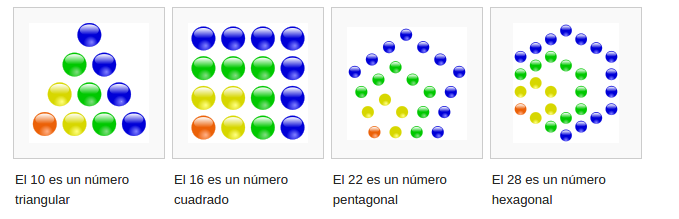
\includegraphics[width=\textwidth]{img/numeros_poligonales.png}
\end{center}

La idea de estos números, más bien de estos esquemas, es que nos permiten representar sucesiones de números que, en cierto modo, serán fáciles de estudiar. 


\subsubsection{Números triangulares}
En el caso de los números triangulares, podemos ver que si contamos los puntos que añadimos en cada nivel al trabajar con los números triangulares tenemos que el número será:
\[S=\sum_{i=1}^ni\]
y tenemos una forma muy sencilla de calcular este número.

Suponemos un cuadrado de dimensión $n$. El total de puntos del cuadrado será $n^2$. Ahora tenemos en cuenta que para nuestro triángulo sólo estamos utilizando la mitad del cuadrado por lo que tendremos $\frac{n^2}{2}$ puntos. Pero al quitar la mitad de puntos estamos quitando toda la parte superior de la diagonal (lo cual es correcto) y la mitad de la diagonal, que debemos recuperar. En total tenemos:
\[S=\frac{n^2}{2}+\frac{n}{2} = \frac{n(n+1)}{2}\]

\subsubsection{Números pentagonales}
 De forma equivalente a lo que hicimos con los números triangulares, podemos trabajar con los números pentagonales obteniendo:
\[S = 1+4+7+10 + ... = \sum_{i=1}^n1+3(i-1) = \frac{n(3n-1)}{2}\]

La demostración de esta fórmula queda como ejercicio para el lector.

\subsection{Números perfectos}
\begin{defn}{Números perfectos}
Un número perfecto es aquel que es igual a la suma de sus divisores.

Son ejemplos de números perfectos el $6=1+2+3$, $28=1+2+4+7+14$.
\end{defn}

Euler llegó a comporbar que los cuatro primeros números perfectos vienen dados por la fórmula: $2^{n-1}(2^n-1)$.

Aunque los griegos dieron mucha importancia a estos números, pues siempre estaban buscando la perfección y relaciones nuevas, a día de hoy no tienen importancia alguna y han quedado sólo como un dato anecdótico.

\subsection{Teoría de divisores}
Euclies fue el primero en dejar constancia de su estudio sobre los números primos en su libro \textbf{Los Elementos}. En el libro prueba diversos teoremas sobre ellos, define los conceptos de máximo común divisor y mínimo común múltiplo y define el algoritmo de Euclides, aún empleado hoy dia.

Uno de los resultados más importantes es el siguiente teorema
\begin{theorem}[Teorema de Euclides]
Existe \textbf{infinitos} números primos
\end{theorem}
\begin{proof}
Consideramos una serie de números primos distintos ordenados de menor a mayor (no tienen por que ser consecutivos): $p1<p_2<p_2<...<p_n$

A partir de estos números calculamos $p_{n+1}$ como el producto de todos más 1, es decir:
\[p_{n+1}=p_1\cdot p_2 \cdot p_3 ... \cdot p_n+1\]

Una vez tenemos calculado $p_{n+1}$ tenemos dos opciones:
\begin{itemize}
\item \textbf{Es primo}

En este caso acabamos de encontrar un nuevo número primo.

\item \textbf{No es primo}

En este caso tendrá factores: $p_{n+1}=q_1\cdot q_2 ... \cdot q_k$, pero podemos observar que:
\[\frac{p_{n+1}}{p_i}=m_i \text{ con resto } r= 1\]
Sin embargo
\[\frac{p_{n+1}}{q_i}=l_i \text{ con resto } r= 0\]

Por tanto es claro que uno de esos $q_i \neq p_j \ \forall i,j$ será un primo nuevo.

\end{itemize}

Es decir, dados $n$ primos siempre podemos encontrar un número primo nuevo. Por tanto queda claro que hay infinitos números primos.

\end{proof}

No obstante, podemos ver que, aunque haya infinitos números primos, la densidad de los mismos va disminuyendo. Así podemos representar la siguiente funciones.
\[ρ(n)=\frac{\#\{q \ : \ 1 < q < n, \ q \text{ es primo }\}}{n}\]
\begin{center}
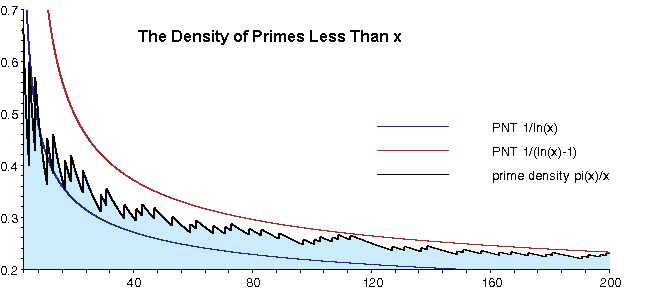
\includegraphics[width=0.8\linewidth]{img/density.png}
\end{center}

\subsubsection{Criba de Erastótenes}
\begin{defn}[Criba de Erastótenes]
La criba de Eratóstenes es un algoritmo que permite hallar todos los números primos menores que un número natural dado n. Se forma una tabla con todos los números naturales comprendidos entre 2 y n, y se van tachando los números que no son primos de la siguiente manera: Comenzando por el 2, se tachan todos sus múltiplos; comenzando de nuevo, cuando se encuentra un número entero que no ha sido tachado, ese número es declarado primo, y se procede a tachar todos sus múltiplos, así sucesivamente. El proceso termina cuando el cuadrado del mayor número confirmado como primo es mayor que n.
\end{defn}

\subsubsection{Máximo común divisor}
Euler nos proporcionó un algoritmo para calcular le máximo común divisor de dos números que aún hoy en día sigue empleándose.

Este método se basa en el siguiente lemma:
\begin{lemma}
Un número $c$ es divisor común a dos números $a>b$ si y sólo si $c$ es divisor común de $a$ y de $r=a\mod b$ 
\end{lemma}
\begin{proof}
Trabajando sobre una cuadrícula, dibujamos un rectángulo de $a$ cuadros de longitud por $b$ de altura.

Una vez tenemos el rectángulo, quitamos del mismo tantos \textbf{cuadrados} de lado $b$ como sea posible. 

Tras esto nos quedará un rectángulo de altura $b$ y base $r$.

\begin{center}
\inputtikz{divisor_comun}
\end{center}

Si tuviésemos un número $c$ que divide a $a$ y a $b$, podríamos haber cubierto todo el rectángulo inicial con cuadrados de tamaño $c$ y, además, podríamos haber cubierto los cuadrados de lado $b$ con cuadrados de tamaño $c$. 

Por tanto, la región sobrante $r\times b$ también se podría cubrir por cuadrados de tamaño $c$ y, por tanto, $c$ tiene que dividir a $r$ también.
\end{proof}

Una vez tenemos claro este lema, el algoritmo de Euclides para calcular el máximo común divisor de dos números consiste en iterar sobre el lema reduciendo el problema a algo cada vez más sencillo.

La idea consiste en que, dados dos números $a>b$ tenemos:
\[c.d.(a,b)=c.d.(b,r_1)=c.d.(r_1,r_2)...\]
\begin{example}
Los divisores comunes de 75 y 28 pueden calcularse como:
\[c.d.(75,28)=c.d.(28,19) = c.d.(19,9)=c.d.(9,1) = c.d.(1,0)\]

Paramos en el momento en que el resto sea 0 con lo que obtenemos que los divisores comunes que estamos buscando son los divisores de 0 y de otro número $c$, es decir, los divisores comunes serán todos los divisores de $c$.
\end{example}

\obs El número $c$ que obtenemos, tal que todos sus divisores son los divisores comunes de $a$ y $b$, es el máximo común divisor de estos números.

Así, acabamos de encontrar un algoritmo para calcular el máximo común divisor entre dos números, conocido como \concept{Algoritmo de Euclides}

Podemos ver el \textbf{algoritmo} trabajando con $a>b>1 \in \nat^+$:
\begin{verbatim}
a = q*b + r;

Mientras r != 0"
    Si r = 0:
        mcd(a,b) = b;
    Si r > 0:
        a = b;
        b = r;
        a = q*b + r;
\end{verbatim}

\subsubsection{Factorizando irracionales}

Veamos qué ocurre si empezamos a trabajar con los números irracionales.

Si dibujamos un cuadrado de base $\sqrt{2}$ y de altura 1, podemos ver que dentro sólo cabe un cuadrado de lado 1 y nos queda un rectángulo de dimensiones $(\sqrt{2}-1)\times 1$.

Puesto que el divisor común que buscamos debe dividir a $\sqrt{2}-1$, por el lemma anterior, entonces podremos dibujar un rectángulo con este valor como lado, que podrá rellenarse con cuadrados de lado $c = c.d.(\sqrt{2},1)$.

Este rectángulo puede dividirse en un cuadrado de lado $\sqrt{2}-1$ y un rectángulo de dimensiones: $(\sqrt{2}-1) \times (1-(\sqrt{2}-1) ) = (\sqrt{2}-1) \times (2 - \sqrt{2})$ que podemos ver que es proporcional al rectángulo con el que empezamos y que debería poder rellenarse con cuadrados de lado $c$.

Por tanto este procedimiento nunca acabará, ya que siempre obtenemos un subrectángulo proporcional al inicial de modo que nunca encontraremos $c$.

Esto supone \textbf{una prueba más de la irracionalidad de $\sqrt{2}$}.

\subsubsection{Métodos de aproximación}
El intento de factorización anterior, si bien no nos aportó información nueva a priori, si que nos ha proporcionado un método de aproximación de irracionales, como $\sqrt{2}$.

Si consideramos el mismo dibujo anterior, con $x = \sqrt{2}$ el lado inferior del rectángulo y $y=x+1$, lo que resta de base al quitar un cuadrado unidad del rectángulo inicial, vemos que obtenemos la iteración:

\[x = 1+y \implies x = 1 + \frac{1}{2+y} = 1 + \frac{1}{1 + \frac{1}{2+y}} = ... \]

Esto nos da un método de aproximación de $x=\sqrt{2}$, para lo que basta tomar un $y$ cualquiera (podemos tomar 0 por comodidad) y tomar la fracción que deseemos. 

Estas fracciones que se prolongan infinitamente son conocidas como \concept{fracciones continuas}

\section{Arquímedes}
\textbf{Arquímedes de Siracusa}, nacido en torno al año 287 a.C. fue un físico, ingeniería|ingeniero, inventor, astrónomo y matemática helénica|matemático griego. Aunque se conocen pocos detalles de su vida, es considerado uno de los científicos más importantes de la Antigüedad clásica. 

Entre sus avances en física se encuentran sus fundamentos en hidrostática, estática (mecánica)|estática y la explicación del principio de la palanca. Es reconocido por haber diseñado innovadoras máquinas, incluyendo arma de asedio|armas de asedio y el tornillo de Arquímedes, que lleva su nombre. 

Experimentos modernos han probado las afirmaciones de que Arquímedes llegó a diseñar máquinas capaces de sacar barcos enemigos del agua o prenderles fuego utilizando una serie de espejos. 


\subsection{Cálculo de π}
Arquímedes desarrolló un procedimiento para aproximar el número π con precisión de tantos decimales como deseemos. No obstante, la mala notación matemática de los griegos hacía los cálculos muy complicados con lo que, a pesar de tener un algoritmo, no llegó a calcular demasiados decimales de π.


La idea consiste en aproximar el perímetro y el área de una circunferencia por medio de polígonos inscritos y circunscritos en la misma.

Vamos a partir de una circunferencia de radio 1 y vamos a considerar los hexágonos inscritos y circunscritos en la misma.

\begin{center}
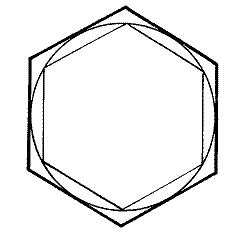
\includegraphics[width=0.3\linewidth]{img/hexagonos.png}
\end{center}

\obs Empleamos el hexágono y no otra figura geométrica por la particularidad de que el radio es igual al lado, lo que nos facilita los cálculos.

\obs En los cálculos que siguen emplearemos letras mayúsculas para referirnos al hexágono mayor (el circunscrito) y minúsculas para el menor (el inscrito).

\obs A lo largo de todo este procedimiento nos apoyaremos en el Teorema de Pitágoras, construyendo triángulos apoyados en medio lado del polígono y con hipotenusa igual al radio.

Podemos escribir las siguientes relaciones, donde $p$ representa el semiperímetro\footnote{Empleamos el semiperímetro en lugar del perímetro puesto que queremos aproximar π directamente, no su doble}:
\[\left\{ \begin{array}{l} 
p_6 = 6x_6 = 6 \frac{1}{2} = 6\\
X_6^2+H_6^2=(2X_6)^2 \implies X_6 = \frac{1}{\sqrt{3}}\\
P_6 = 6X_6 = \frac{6}{\sqrt{3}} = 2\sqrt{3}
\end{array}\right.\]

Podemos tratar de establecer una relación entre los lados del polígono inscrito y el circunscrito.

\[\frac{X_6}{x_6} = 2\sqrt{3} = \frac{H_6}{h_6} = \frac{1}{\sqrt{1-x_6^2}}\]

De forma general, deducimos la fórmula:
\[X_n=\frac{x_n}{\sqrt{1-x_n^2}}\]

Ahora deberíamos tomar un polígono con más lados de forma que tengamos mayor precisión. Lo más cómodo será considerar un dodecaedro.

Empezamos buscando la relación entre la longitud del lado del hexágono y del dodecaedro de forma general. 

\[\left\{ \begin{array}{l}
x_n^2 + (1-h_n)^2 = (2x_{2n})^2 \\
x_n^2+(1-\sqrt{1-x_n^2})^2 = 4x_{2n}^2\\
x_n^2+1+1-x_n^2 - 2 \sqrt{1-x_n^2} = 4x_{2n}^2\\
\end{array}\right. \implies 2x_{2n}^2 = \frac{x_n^2}{1+\sqrt{1-x_n^2}}\]

Ahora tomamos la relación entre $x_n$ y $X_n$ y escribimos:
\[X_{2n} = \frac{x_{2n}}{\sqrt{1-x_{2n}^2}} = \frac{x_n}{1+\sqrt{1-x_n^2}}\]

Una vez tenemos escritos los lados, podemos calcular los semiperímetros.
\[p_n = n x_n\]
\[P_n =nX_n = n \frac{x_n}{1-x_n^2}\]
\[p_{2n}=2nx_{2n} = n\left(\frac{1}{2} \frac{x_n^2}{1+\sqrt{1-x_n}}\right)^{\frac{1}{2}}\]
\[P_{2n} = 2nX_{2n} = 2n \frac{x_n}{1+\sqrt{1-x_n}}\]

Jugando con estas ecuaciones podemos llegar a:
\[P_{2n}=\frac{2P_n\cdot p_n}{P_n + p_n}, \ \ \ p_{2n}=\sqrt{p_nP_{2n}}\]

A partir de estas relaciones podemos iterar, comenzando con hexágono cuyos perímetros sabemos calcular, avanzando hacia una cota cada vez más aproximada de π.


\chapter{Ejercicios}
\section{Ejercicios mandados en clase}
\begin{problem}[1]
Demostrar que cada uno de los ángulos de un triángulo equilátero es de $\frac{π}{3}$.
\solution
\end{problem}

\begin{problem}[2]
Demostrar que cada una semicircunferencia, cualquier punto de la misma nos sirve para construir un triángulo rectángulo (con el ángulo recto en el punto dado) que tiene como base el diámetro de la circunferencia.
\solution
\end{problem}

\begin{problem}[3]
Demostrar que dado el triángulo del ejercicio anterior, el ángulo formado entre base y el segmento que une el centro con el punto de la semicircunferencia es el doble del ángulo izquierdo del triángulo.
\solution
\end{problem}

%% Apéndices (ejercicios, exámenes)
% \appendix





% -*- root: ../HistoriaMatematicas.tex -*-
\section{Hoja 1}

Los ejercicios que vienen ahora requieren más búsqueda por internet que otra cosa.

Al final de cada ejercicio añadiré una lista con los link de los que he obtenido la información.

\subsection{Babilonia, Egipto y China}
\begin{problem}[1]
Ejemplos de números escritos por el método babilónico de cuñas

\solution

El sistema de numeración mesopotámica (también llamado numeración babilónica) es un sistema de representación de los números en la escritura cuneiforme de varios pueblos de Mesopotamia, entre ellos los sumerios, los acadios y los babilonios.

Este sistema apareció por primera vez alrededor de 1800-1900  a. C. También se acredita como el primer sistema de numeración posicional, es decir, en el cual el valor de un dígito particular depende tanto de su valor como de su posición en el número que se quiere representar. Esto era un desarrollo extremadamente importante, porque, antes del sistema lugar-valor los técnicos estaban obligados a utilizar símbolos únicos para representar cada potencia de una base (diez, cien, mil, y así sucesivamente), llegando a ser incluso los cálculos más básicos poco manejables.

Aunque su sistema tenía claramente un sistema decimal interno prefirieron utilizar 60 como la segunda unidad más pequeña en vez de 100 como lo hacemos hoy. Más apropiadamente se considera un sistema mixto de las bases 10 y 60. Un valor grande al tener como base sesenta es el número da como resultado un guarismo más pequeño y que además se puede dividir sin resto por dos, tres, cuatro, cinco, y seis, por lo tanto también diez, quince, veinte, y treinta. Solamente dos símbolos usados en una variedad de combinaciones eran utilizados para denotar los 59 números. Un espacio fue dejado para indicar un cero (siglo III a. C.), aunque idearon más adelante una forma de representar un lugar vacío.

La teoría más comúnmente adoptada es que el 60, un número compuesto de muchos factores, fue elegido como base debido a su factorización 2×2×3×5, que lo hace divisible por 1, 2, 3, 4, 5, 6, 10, 12, 15, 20, y 30. De hecho, es el entero más pequeño divisible por todos los enteros del 1 al 6.

Los enteros y las fracciones eran representados de la misma forma: el punto separador de enteros y fracciones no era escritas, sino que quedaban aclaradas por el contexto.


\begin{center}
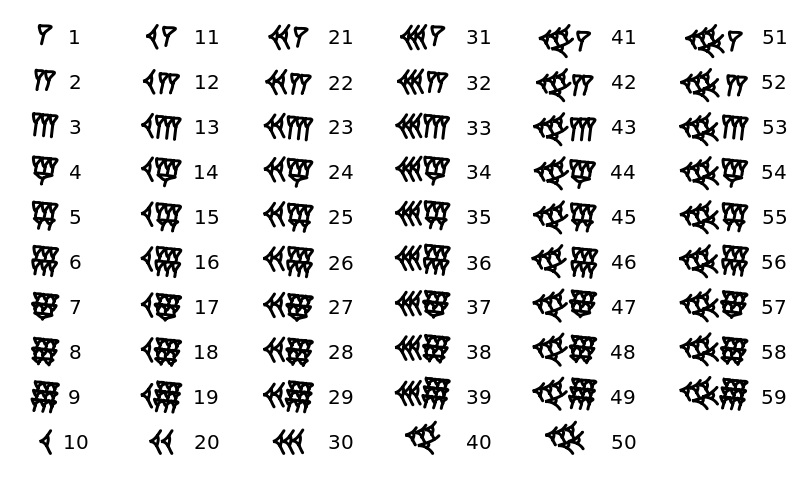
\includegraphics[width=0.8\linewidth]{img/numeros_babilonicos.png}
\end{center}


Por ejemplo, el número 53 en numeración babilónica se representaba utilizando cinco veces el símbolo correspondiente a 10, y 3 veces el símbolo correspondiente a 1, como se puede ver en la imagen superio o solamente el 50 y el 3.

\begin{itemize}
\item \href{https://es.wikipedia.org/wiki/Numeracion_babilonica}{Wikipedia}
\end{itemize}
\end{problem}

\begin{problem}[2]
Ejemplos de números escritos por el método chino tradicional usado hoy día

\solution

La forma clásica de escritura de los números en China se empezó a usar desde el 1500 A.C. aproximadamente. Es un sistema decimal estricto que usa las unidades y los distintas potencias de 10. Utiliza los ideogramas de la figura

\begin{center}
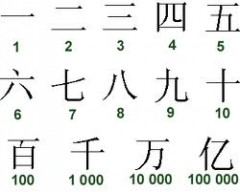
\includegraphics[width=0.4\linewidth]{img/numeracion_china.jpg}
\end{center}

y usa la combinación de los números hasta el diez con la decena, centena, millar y decena de millar para según el principio multiplicativo representar 50, 700 ó 3000. El orden de escritura se hace fundamental,ya que 5 10 7 igual podría representar 57 que 75.

En la

\begin{center}
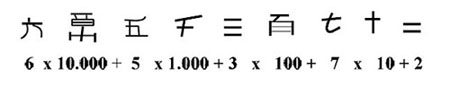
\includegraphics[width=0.6\linewidth]{img/ejemplo_num_chino.jpg}
\end{center}


\begin{itemize}
\item \href{http://www.sectormatematica.cl/historia/chino.htm}{Página random}
\item \href{https://es.wikipedia.org/wiki/Numeracion_china}{Wikipedia}
\end{itemize}
\end{problem}

\begin{problem}[3]
¿Cuál es la mayor terna pitagórica que conocían los babilónicos? Extraer la información de la tablilla Plimton 322

\solution

Plimpton 322 es una tablilla de barro de Babilonia, que destaca por contener un ejemplo de las matemáticas babilónicas. Tiene el número 322 en la colección GA Plimpton en la Universidad de Columbia. Esta tableta, se cree que fue escrita cerca de 1800 a. C., tiene una tabla de cuatro columnas y 15 filas de números en escritura cuneiforme de la época.

Esta tabla muestra lo que ahora se llaman ternas pitagóricas, es decir, números enteros a, b, c que satisfacen $a^2+b^2=c^2$. Las tripletas son demasiadas como para haber sido construidas por fuerza bruta (es decir, hechas a mano probando valores).

Desde una perspectiva moderna, un método para construir tales tripletas es un primer logro significativo, conocido antes sólo entre los griegos . Al mismo tiempo, hay que recordar que el autor de la tableta era un escriba, más que un matemático profesional, se ha sugerido que uno de sus objetivos pueden haber sido producir ejemplos para problemas escolares.

Aunque la tableta se interpretó en el pasado como una tabla trigonométrica, más recientemente se han publicado trabajos que ven esto como un anacronismo, y le dan una función diferente.

El contenido principal de Plimpton 322 es una tabla de números, con cuatro columnas y quince filas, en notación sexagesimal babilónica. La cuarta columna es sólo un número de fila, ordenada del 1 al 15. Las segunda y tercera columnas son completamente visible en la tableta sobreviviente. Sin embargo, el borde de la primera columna se ha roto, y existen dos extrapolaciones consistentes que dan los dígitos faltantes que podrían haber sido; estas interpretaciones difieren sólo en si cada número comienza con un dígito adicional igual a 1 o no. Con las diferentes extrapolaciones mostradas en paréntesis, estos números son:

Si traducimos la tabla literalmente tenemos
\begin{center}
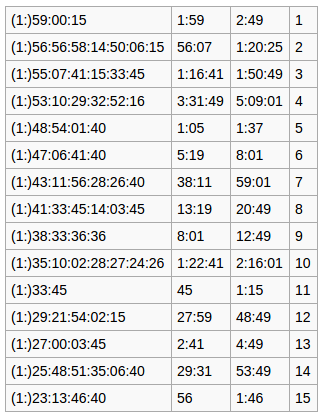
\includegraphics[width=0.5\linewidth]{img/plimton_literal.png}
\end{center}

que se interpreta como:
\begin{center}
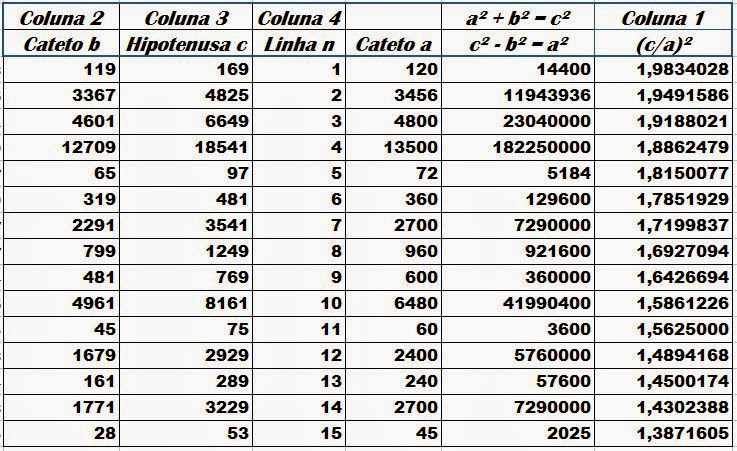
\includegraphics[width=0.8\linewidth]{img/plimton322.jpg}
\end{center}

En respuesta al ejercicio, la terna más grande que conocían es
\[(13500, 12709, 18541)\]

\begin{itemize}
\item \href{https://es.wikipedia.org/wiki/Plimpton_322}{Wikipedia}
\end{itemize}

\end{problem}

\begin{problem}[4]
Raíz cuadrada por el \textbf{método de Heron}.

Sea
\[x_{n+1} = \frac{1}{2} \left(x_n + \frac{R}{x_n} \right)\]
demostrar que existe el límite y que la serie converge a  $\sqrt{R}$. Describir el conjunto de los datos iniciales que llevan a convergencia.
\solution

\doneby{Pedro}

El método de Herón que menciona el ejercicio es un algoritmo que nos permite calcular raíces cuadradas (más bien aproximaciones a las mismas).

Para estudiar la convergencia podemos buscar el punto fijo de la ecuación.
\[x_n = \frac{1}{2} \left(x_n+\frac{R}{x_n}\right) \implies \frac{1}{2}x_n=\frac{1}{2}\frac{R}{x_n} \implies x_n^2=R \implies x_n = \sqrt{R}\]

El método funcionará (convergerá a lo que deseamos) si
\[\norm{f(x)-f(y)} \leq K \norm{x-y} \text{ con } f(x)=\frac{1}{2} \left( x + \frac{R}{x} \right)\]

Podemos ver que
\[\norm{f(x)-f(y)} = \frac{R}{2}\left(\frac{1}{x}-\frac{1}{y}\right)\]

Sea $x$ la solución, es decir $x=\sqrt{R}$ podemos escribir $y=x+ε$ lo que nos lleva a:
\[\norm{f(x)-f(y)} = \frac{R}{2}\left(\frac{1}{x}-\frac{1}{x+ε}\right) = \frac{R}{2} \left( \frac{ε}{x^2+xε} \right)<Kε\]

Para garantizar la desigualdad necesitamos que el denominador sea mayor que 1, es decir, basta con tomar
\[x^2+xε > 1 \implies ε > \frac{1-x^2}{x}=\frac{1-R}{\sqrt{R}}>\frac{1}{\sqrt{R}}-\sqrt{R}\]

Por tanto basta con que tomemos un punto $y>x+\frac{1}{\sqrt{R}}-\sqrt{R} = \frac{1}{\sqrt{R}}$.

Cuando $R$ sea bastante grande, prácticamente nos bastará con tomar cualquier número positivo.


\end{problem}

\subsection{Grecia}
\begin{problem}[5]
Elaborar una tabla con el alfabeto griego, los símbolos, la fonética y el nombre y pronunciación usual de cada letra.

\obs Epsilon y eta; i e ípsilon; o y omega; zeta y theta; nu, xi, phi, psi y los diptongos ai=e, ei=i

\solution

El alfabeto griego es un alfabeto de veinticuatro letras utilizado para escribir la lengua griega. Desarrollado alrededor del siglo IX a. C. a partir del alfabeto consonántico fenicio, los griegos adoptaron el primer alfabeto completo de la historia, entendiéndolo como la escritura que expresa los sonidos individuales del idioma, es decir que prácticamente a cada vocal y cada consonante corresponde un símbolo distinto.

\begin{center}
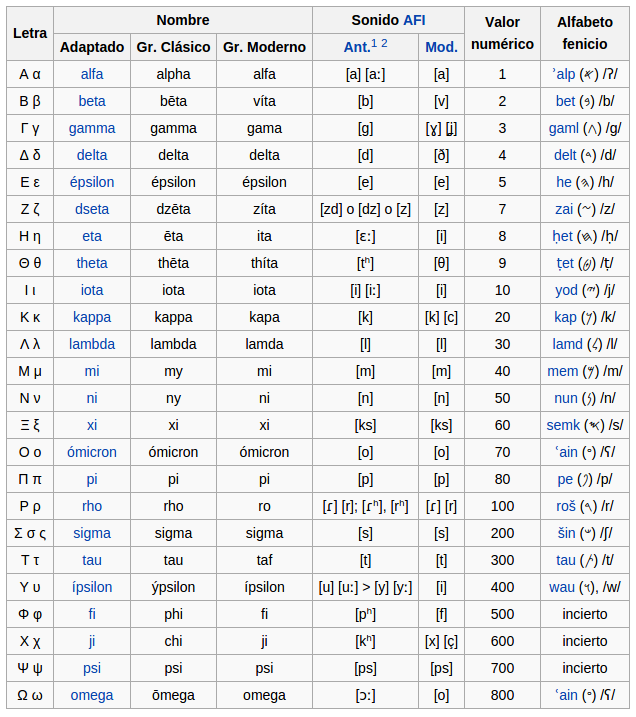
\includegraphics[width=0.5\linewidth]{img/alfabeto_griego.png}
\end{center}


Su uso continúa hasta nuestros días, tanto como alfabeto nativo del griego moderno como a modo de crear denominaciones técnicas para las ciencias, en especial la lógica, la matemática, la física, la astronomía y la informática.


\begin{itemize}
\item \href{https://es.wikipedia.org/wiki/Alfabeto_griego}{Wikipedia}
\end{itemize}


\end{problem}

\subsection{Thales}
\begin{problem}[6]
\ppart Demostrar que en un triángulos con dos lados iguales hay dos ángulos iguales y viceversa

\ppart Demostrar que la suma de ángulos de un triángulo es un ángulo plano

\ppart Demostrar el siguiente teorema de Tales: el ángulo inscrito en una semicircunferencia es recto. Demostrar el inverso

\ppart Demostrar que el ángulo inscrito en una circunferencia vale la mitad del ángulo central correspondiente

\solution

\doneby{Pedro}

\spart

Si tomamos un triángulo isósceles podemos dividirlo en dos triángulos rectángulos dibujando la altura sobre el lado desigual.

Asumiendo que los lados son iguales, vamos a obtener dos triángulos con los tres lados iguales por lo que también tendrán los ángulos iguales.

\spart

Basándonos en el Teorema de Tales tenemos:

\begin{center}
\inputtikz{suma_angulos_triangulo}
\end{center}

donde las rectas del mismo color son paralelas y los del mismo color iguales por el teorema de tales.

Viendo esto y sabiendo que un ángulo llano tiene 180 grados, es sencillo ver que la suma de los ángulos es 180.

\spart


\end{problem}

\subsection{Pitágoras}
\begin{problem}[7]
Escribir la definición de las ternas pitagóricas. Describir todas las ternas pitagórigas mediante dos fórmulas. Listar todas aquellas ternas que tienen todos los números menores que 500

\solution

Una terna pitagórica consiste en una tupla de tres enteros positivos a, b, c que cumplen que a² + b² = c². El nombre deriva del teorema de Pitágoras, el cual plantea que en cualquier triángulo rectángulo, se cumple que x² + y² = z² (siendo x e y las longitudes enteras de sus catetos y z la de la hipotenusa). En sentido contrario también se cumple, o sea, cualquier terna pitagórica se puede asociar con las longitudes de dos catetos y una hipotenusa, formando un triángulo rectángulo.

Las ternas pitagóricas suelen representarse como (a,b,c).



\begin{itemize}
\item \href{https://conlamenteabierta.wordpress.com/2010/02/18/diofanto-y-las-tripletas-pitagoricas/}{CONLAMENTEABIERTA}
\end{itemize}
\end{problem}

\begin{problem}[8]
Método de Diofanto para calcular las ternas pitagóricas. Describir el método y el uso de los números fraccionarios.

Aplicar el método disparando de $N=(0,-1)$ o desde $N'=(1,0)$. Comparar

\solution

Una relación que nos dio Diofanto para calcular ternas pitagóricas es:

\[\left\{ \begin{array}{l} a=p^2-q^2 \\ b=2pq \\ c=p^2+q^2 \end{array} \right.\]

Considerando los datos iniciales del enunciado tenemos:
\[N \to (-1,0,1); \ \ N' \to (-1,0,1)\]

Obtenemos el mismo resultado en ambos casos pues las magnitudes aparecen elevadas al cuadrado.

\begin{itemize}
\item \href{https://en.wikipedia.org/wiki/Diophantus_II.VIII}{Wikipedia en inglés}
\end{itemize}
\end{problem}

\begin{problem}[9]
Leer el capítulo 1 de Stillwell (3rd Edition). Hacer los ejercicios 1.2.\{1,3,4\}, 1.3.\{1,2,3\}.

Especialmente el último

\solution

\doneby{Pedro}

\begin{enumerate}
\item \textbf{Si $(a,b,c)$ es una terna pitagórica y $a,b,c$ no tienen factor común entonces $a,b$ son uno par y otro impar}

Si $a,b$ son pares entonces sus cuadrados también lo son, la suma de ellos también, por tanto lo es $c^2$ y deberá serlo $c$ lo que nos lleva a una contradicción pues en ese caso el 2 sería un factor común a los tres elementos de la terna y estamos suponiendo que no hay factor común.

Si $a,b$ fuesen impares, por un razonamiento similar al anterior llegaríamos a que $c$ debe ser par. Entonces podemos escribir:
\[\left\{\begin{array}{l}
a=2n+1 \\
b=2m+1\\
c=2l
\end{array} \text{ con } n,l,m \in \nat\right. \implies 4n^2+4n+1 +4m^2+4m+1 = 4l^2 \implies \atop \implies l^2=n^2+m^2+n+m+\frac{1}{2} \implies l \notin \nat\]

\item \textbf{A partir del método para calcular coordenadas racionales de la circunferencia unidad deriva la fórmula para calcular ternas pitagóricas}

Recordamos que este método consistía en dibujar rectas de pendiente racional que pasasen por el $(-1,0)$ y encontrar la intersección de estas con la circunferencia.

Haciendo esto, tomando $y=t(x+1)$ obtenemos puntos de la forma:
\[\left(\frac{1-t^2}{1+t^2}, \frac{2t}{1+t^2}\right)\]

Con este método estamos generando ternas pitagóricas de la forma:
\[\left\{\begin{array}{l}
a=\frac{1-t^2}{1+t^2} \\
b=\frac{2t}{1+t^2}\\
c=1
\end{array}\right.\]

Como la fórmula que nos piden obtener servía para generar ternas con coeficientes enteros podemos multiplicar todos los términos por $(1+t^2)$ obteniendo
\[\left\{\begin{array}{l}
a=1-t^2 \\
b=2t\\
c=1+t^2
\end{array}\right.\]

Si en lugar de trabajar con la circunferencia unidad lo hubiésemos hecho con otra de radio $r$ el punto obtenido sería:
\[\left(\frac{r^2-t^2}{r^2+t^2}, \frac{2tr}{r^2+t^2}\right)\]
con lo que llegamos a:
\[\left\{\begin{array}{l}
a=r^2-t^2 \\
b=2tr\\
c=r^2+t^2
\end{array}\right.\]

\item \textbf{Comprueba que cuando una solución racional de las ecuaciones de Diofanto es conocida, el método os da todas las soluciones racionales de cualquier ecuación cuadrática con coeficientes racionales}

El método de Diofanto se aplica cuando tenemos ecuación cuadrática de la forma $Ax^2+By^2=C$ con $A,B,C \in \rac$ y de la que conocemos una solución trivial $(p,q)$ con $p,q \in \rac$.

La idea consiste en ver la ecuación como una curva en el espacio y trazar una recta con pendiente $t \in \rac$ desde la solución trivial e intersecarla de nuevo con la curva, con lo que obtendremos otra solución.

La recta será $y=t(x-p)+q$. Para encontrar la intersección vemos que

\[Ax^2 + B\left(t(x-p)+q\right)^2 = C \iff Ax^2+Bt^2(x-p)^2 +Bq^2+2Bt(x-p)q=C \iff\]
\[\iff x^2 (A+Bt^2) + x (2Btq-2Bt^2p) + \left(Bq^2-Bt^2p^2-2Btq-C\right) = 0\]

Resolviendo la ecuación temeos:
\[x= \frac{-2Btq+2Bt^2p \pm \sqrt{4B^2t^2(q^2+t^2p^2-2tpq)-4ABq^2+4ABt^2p^2-8ABtq+4AC\atop -4B^2t^2q^2+4B^2t^4p^2+8B^2t^3q+4Bt^2C}}{2(A+Bt^2)}=\]
\[=\frac{-Btq+Bt^2p \pm \sqrt{4B^2t^4p^2-ABq^2+ABt^2p^2-4ABtq+AC +Bt^2C}}{A+Bt^2}\]

Sabiendo que el punto $(p,q)$ es solución de la ecuación diofántica podemos escribir
\[x=\frac{-Btq+Bt^2p \pm \sqrt{4B^2t^4p^2-A(C-Ap^2)+ABt^2p^2-4ABtq+AC +Bt^2C}}{A+Bt^2}=\]
\[=\frac{-Btq+Bt^2p \pm \sqrt{4B^2t^4p^2+A^2p^2+ABt^2p^2-4ABtq +Bt^2(Ap^2+Bq^2)}}{A+Bt^2}=\]
\[=\frac{-Btq+Bt^2p \pm \sqrt{4B^2t^4p^2+A^2p^2+2ABt^2p^2-4ABtq +B^2t^2q^2}}{A+Bt^2}=\]
\[=\frac{-Btq+Bt^2p \pm \sqrt{(Ap+2Bt^2q)^2-2ABt(tp^2+q)+B^2t^2q^2}}{A+Bt^2}=\]
\[=\frac{-Btq+Bt^2p \pm (Ap+2Bt^2q)-Btq}{A+Bt^2}\]
que podemos comprobar es un valor racional.


\item \textbf{Comprueba que cualquier triángulo rectángulo puede ser aproximado con tanta precisión como queramos por uno de lados racionales.}



\end{enumerate}


\end{problem}

\begin{problem}[10]
Sea $(a,b,c)$ una terna pitagórica generada por $(p,q)$ con $a,b,c,p,q$ enteros positivos, demostrar que si $p=q+1$, entonces $c=b+1$.

\solution
\doneby{Pedro}

Recordemos que las ternas pitagóricas podrían generarse a partir de dos enteros $p$ y $q$ considerando:
\[\left\{ \begin{array}{l} a=p^2-q^2 \\ b=2pq \\ c=p^2+q^2 \end{array} \right.\]

Si tomamos $p=q+1$ obtendremos
\[c=p^2+q^2=(q+1)^2-q^2=1+2q+2q^2\]
Por otro lado tendremos:
\[b=2pq=2(q+1)q=2q^2+2q\]
Así es sencillo ver que
\[c=b+1\]
\end{problem}

\begin{problem}[11]
Demuestra que al menos uno de los tres términos de una terna pitagórica es par.

\solution

\doneby{Pedro}

Si ninguno fuese par, tendríamos que todos los cuadrados son impares y al escribir:
\[a^2+b^2=c^2\]
tendríamos que la suma de dos números impares es impar, afirmación que es totalmente falta.
\end{problem}

\begin{problem}[12]
\ppart En toda terna pitagórica generada por $p$ y $q$ siendo ambos positivos y $p>q$, mediante la fórmula simple
\[F(p,q)=(p^2-q^2,2pq,p^2+q^2)\]
al menos uno de los tres números resultantes es divisible por 3.

\ppart En toda terna pitagórica $(a,b,c)$ generada por $p$ y $q$ como antes, al menos uno de los tres números resultantes es divisible por 5
\solution

\doneby{Pedro}

\spart

Supongamos que ninguno de los números es múltiplo de 3, es decir:
\[\left\{ \begin{array}{l} a=p^2-q^2=3m+i \\ b=2pq=3n+j \\ c=p^2+q^2=3h+k \end{array} \right. \text{con } i,j,k = 1 \text{ ó } 2\]

Cuando pasemos a corroborar que se satisface la ecuación de Pitágoras tendremos:
\[9m^2+i^2-6mi+9n^2+j^2+6nj=9h^2+k^2+6hk\]

Podemos ver que $i^2,j^2,k^2=3l+1$ con $l=1 \text{ ó } 0$.

Por tanto, agrupando los múltiplos de 3 a ambos lados nos quedará:
\[3x+2=3y+1\]
igualdad que no puede satisfacerse siendo $x,y$ enteros.

\spart

Repetimos el mismo procedimiento del apartado anterior.

Supongamos que ninguno de los números es múltiplo de 5, es decir:
\[\left\{ \begin{array}{l} a=p^2-q^2=5m+i \\ b=2pq=5n+j \\ c=p^2+q^2=5h+k \end{array} \right. \text{con } i,j,k = 1,2,3 \text{ ó } 4\]

Cuando pasemos a corroborar que se satisface la ecuación de Pitágoras tendremos:
\[25m^2+i^2-10mi+25n^2+j^2+10nj=25h^2+k^2+10hk\]

Podemos ver que $i^2,j^2,k^2=5l+t$ con $t=1 \text{ ó } 4$.

Por tanto, agrupando los múltiplos de 5 a ambos lados nos quedará:
\[5x+u=5y+v\]

Veamos todos los casos posibles.
\begin{center}
\begin{tabular}{|c|c|c|}
\hline
u & v & Validez\\
\hline
\hline
2 & 1 & No \\
 \hline
5 & 1 & No \\
 \hline
3 & 1 & No \\
\hline
2 & 4 & No \\
 \hline
5 & 4 & No \\
 \hline
3 & 4 & No \\
\hline
\end{tabular}
\end{center}

Podemos ver que en ningún caso se puede satisfacer la ecuación.

\end{problem}

\begin{problem}[13]
Hallar una terna pitagórica especial que genere un triángulo rectángulo cuyas alturas sean, todas ellas, números enteros positivos
\solution

\doneby{Pedro}

Puesto que hablamos de triángulos rectángulos, los lados $a$ y $b$ ya son alturas entre ellos.

Por tanto, toda terna pitagórica nos da un triángulo en el que dos de sus alturas son números enteros positivos.

Sabemos calcular el área de un triángulo rectángulo de dos formas distintas que deben dar el mismo valor:
\[A = \frac{bc}{2} = \frac{ah}{2} \implies h = \frac{bc}{a}\]

donde $h$ es justo la altura de la que no podemos garantizar que sea entera.

Tanteando un poco parece lógico tomar valores de $p$ y $q$ que tengan un factor común y si ese factor común es el $2$ parece que será más sencillo puesto que al generar la $b$ nos aparece un 2.

Finalmente, por la cuenta de la vieja podemos ver que
\[p=10, \ q=6\left\{ \begin{array}{l} a=p^2-q^2=64=2^(6) \\ b=2pq=120=2^3(5\cdot 3) \\ c=p^2+q^2=136=2^3\cdot 17 \end{array} \right. \]

Y podemos comprobar fácilmente que este caso satisface que $h=\frac{bc}{a} \in \nat$.
\end{problem}

\begin{problem}[14]
Hacer los ejercicios 1.5.\{1,2\} del Stillwell
\solution

\doneby{Pedro}

Justo estos ejercicios no existen en la edición que tengo.

\begin{enumerate}
\item \textbf{Comprueba que los tres triángulso obtenidos al dibujar la altura de un triángulo rectángulo respecto al ángulo recto son similares y, por tanto, tenemos una nueva prueba del teorema de Pitágoras igualando los ratios correspondientes a cada lado}

\end{enumerate}
\end{problem}

\begin{problem}[15]
Teorema de Pitágoras. Enunciado e interpretación geométrica. Dos pruebas por la técnica de recorte de figuras (tangram)
\solution

Este ejercicio esta resuelto en la teoría, concretamente en los apartados \ref{sec:Prueba1} y \ref{sec:Prueba2}
\end{problem}

\begin{problem}[16]
Teorema de Pitágoras. Enunciado y prueba por el Método de Semejanzas. Obtener los dos teoremas de la altura.

\solution

Este ejercicio está resuelto en la teoría, concretamente en \ref{sec:Prueba3}


\end{problem}


\subsection{Construcciones geométricas}
\begin{problem}[17]
\ppart Construcciones con regla y compás: Dividir un segmento en 2,3,...,p partes iguales.
\ppart Hallar un trozo de segmento dado en proporción m/n al total
\ppart Hallar un trozo de un segmento dado en la proporción $\frac{1}{\sqrt{2}}$

\solution
\doneby{Pedro}

\spart

Eso lo aprendimos en las primeras clases de dibujo técnico de bachillerato. Basta con apoyarnos en un segmento auxiliar de longitud $p$ unidades, donde la unidad puede ser de cualquier tamaño.

Supongamos que queremos dividir el segmento $\overline{AB}$ en 5 partes iguales. Para ello realizamos la siguiente construcción.

\begin{center}
\inputtikz{dividir_segmento}
\end{center}

\spart

Basta con repetir el procedimiento del apartado anterior, donde la recta $\overline{AG}$ sólo tendría un punto intermedio que estaría a distancia $n$ de $A$ y $m$ de $G$.

En el fondo en el apartado anterior hemos dividido el segmento en trozos de segmento en la proporción $\frac{\overline{AC}}{\overline{AG}}$.


\spart

Lo que tenemos que hacer es encontrar la forma geométrica de relacionar una longitud $l$ con $\sqrt{2}l$, cosa que es sencilla a través del cuadrado.

Por tanto, dado un segmento cualquiera podemos construir un cuadrado que tenga al segmento por lado y la diagonal será el resultado que buscamos


\end{problem}

\begin{problem}[18]
Construcciones con regla y compás. Construir un cuadrado equivalente a un rectángulo dado. Construir un cuadrado de área dada.
\solution

\doneby{Pedro}

\begin{minipage}{0.47\textwidth}
\begin{center}
\inputtikz{cuadrado_equivalente_rectangulo}
\end{center}
\end{minipage}
\begin{minipage}{0.52\textwidth}

El teorema de la altura de Tales nos garantiza que
\[h^2=l_1l_2\]
por lo que es evidente que el rectángulo negro y el cuadrado verde tienen el mismo área.
\end{minipage}

Para construir ahora un cuadrado conociendo el área lo más sencillo que podemos hacer es construir un rectángulo que tenga ese área y transformarlo en un cuadrado equivalente con el procedimiento que acabamos de ver

El rectángulo más sencillo de construir dada su área es aquel que tiene por base un segmento de longitud igual al valor del área que queremos y altura 1.

\end{problem}

\begin{problem}[19]
Hacer los cálculos de longitudes y áreas en los polígonos regulares de 3, 4, 6 y 8 lados. Intentarlo con el pentágono.
\solution

\end{problem}

\begin{problem}[20]
Problemas de axiomas y modelos. Examinar si en los postulados de Euclides se puede cambiar recta por punto y viceversa y obtener unos axiomas válidos
\solution

\doneby{Pedro}

Los postulados de Euclides son:

\begin{enumerate}
\item Dos puntos cualesquiera determinan un segmento de recta.
\item Un segmento de recta se puede extender indefinidamente en una línea recta.
\item Se puede trazar una circunferencia dados un centro y un radio cualquiera.
\item Todos los ángulos rectos son iguales entre sí.
\item Postulado de las paralelas. Si una línea recta corta a otras dos, de tal manera que la suma de los dos ángulos interiores del mismo lado sea menor que dos rectos, las otras dos rectas se cortan, al prolongarlas, por el lado en el que están los ángulos menores que dos rectos.
\end{enumerate}

Si intercambiamos los términos recta y punto obtenemos:

\textbf{\textcolor{red}{WTF???}}

\end{problem}


\begin{problem}[21]
Explicar cuál es el problema histórico del V Postulado
\solution

El quinto postulado de Euclides dice: ``Si una recta al incidir sobre dos rectas hace los ángulos internos del mismo lado menores que dos ángulos rectos, las dos rectas prolongadas indefinidamente se encontrarán en el lado en el que están los ángulos menores que dos rectos.''

Unos 22 siglos después de que se escribieran los Elementos por fin se llega a una conclusión: el V postulado es independiente de los otros cuatro. Y se llega a esta respuesta mediante un camino sorprendente. La prueba de la independencia del V postulado lleva implícita la posibilidad de que existan geometrías en los que no se cumple este postulado. Dicho de otro modo: desde el punto de vista lógico no hay contradicción ninguna en suponer que por un punto exterior a una recta puedan pasar más de una paralela a la recta, o incluso ninguna.

Parece difícil comprender esta afirmación, puesto que en la experiencia común sabemos que (excepto errores de dibujo), el V postulado es cierto. Para comprenderlo debemos hacer un esfuerzo de abstracción por intentar olvidar nuestro significado intuitivo de qué es una recta y acudir únicamente a las definiciones de Euclides.

En el siglo XIX se da conclusión al problema de la independencia del V postulado. Lo hacen de manera independiente Bolyai y Lobachevsky, aunque Gauss ya había resuelto el problema con anterioridad (eso sí, no había publicado sus resultados, y la paternidad del descubrimiento fue para los otros dos geómetras). La idea es muy simple: en Matemática no está permitido llegar a una contradicción, es decir, obtener un resultado que sea exactamente la negación de otro resultado. No puede obtenerse que partiendo de las mismas hipótesis sea cierto, a la vez, que (por ejemplo) dos rectas se corten y que esas dos mismas rectas no se corten. Se llegaría a la conclusión de que (de no haber cometido errores de razonamiento, claro) alguna de las hipótesis ha de ser falsa.

La idea que dio solución al problema es la siguiente: si el V postulado depende de los otros cuatro, es que no nos hace falta incluirlo entre nuestras hipótesis (postulados). Así que en el desarrollo de la teoría, tarde o temprano, aparecerá en forma de teorema. Ahora bien, si eliminamos dicho postulado y le añadimos su negación, de ser cierto que el postulado V depende de los otros, llegaremos a demostrarlo, y con ello tendremos que tanto una proposición (el V postulado) como su contraria (la negación del V postulado que ahora lo sustituye) son ciertas. Habremos pues llegado a una contradicción, algo que no es admisible. Alguna de las hipótesis tiene que ser falsa, y esta ha de ser la nueva que se ha introducido, pues es la única que choca contra nuestra intuición (las demás sabemos que son ciertas porque ya lo eran en la geometría de Euclides).

En contra de lo que pudiera pensarse, con este método no se llegó a contradicción alguna. Es más, se llegó a demostrar que las geometrías así obtenidas por Bolyai y por Lobachevsky eran consistentes (lo que quiere decir que no contenían contradicción lógica ninguna). Además hay diferentes formas de negar el V postulado (por un punto exterior a una recta no pasa una única recta paralela a la misma) y así diferentes geometrías no euclídeas: por ejemplo, si decimos que no pasa ninguna recta, se obtiene la geometría esférica, que ya hemos presentado, y si decimos que pasan infinitas se obtiene la geometría hiperbólica, la de Lobachevsky.

\obs Un ejemplo de geometría en la que no se cumple el V Postulado es la \textbf{geometría hiperbólica} pues esta satisface sólo los cuatro primeros postulados de Euclides y tiene curvatura negativa (en esta geometría, por ejemplo, la suma de los tres ángulos interiores de un triángulo es inferior a 180°).

\begin{itemize}
\item \href{https://es.wikipedia.org/wiki/Quinto_postulado_de_Euclides}{Wikipedia}
\end{itemize}
\end{problem}

\subsection{Aritmética}
\begin{problem}[22]
Calcular la fórmula de los números triangulares y pentagonales
\solution

\doneby{Pedro}

Por comodidad vuelvo a añadir aquí la imagen que representa la construcción de los números figurados.

\begin{center}
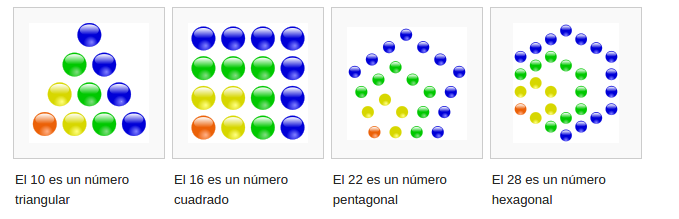
\includegraphics[width=\textwidth]{img/numeros_poligonales.png}
\end{center}

Para los números triangulares es sencillo ver que en la iteración $n$ estamos añadiendo $n$ puntos al conjunto por lo que el n-ésimo número triangular se calcula como:
\[\sum_{i=1}^ni=\frac{n(n+1)}{2}\]

Para los números pentagonales podemos ver que en cada iteración estamos añadiendo $k+3$ puntos, donde $k$ es el número de puntos que teníamos en la iteración anterior. Por tanto, el n-ésimo número pentagonal se calcula como:
\[n+\sum_{i=1}^n(i-1)3 = n+3\sum_{i=1}^ni-3n=-2n+3\frac{n(n+1)}{2} = \frac{3n^2}{2}-\frac{n}{2}\]
\end{problem}

\begin{problem}[23]
EUCLIDES: Números primos: algoritmo para la descomposición de un número entero positivo en producto de números primos. Demostración de unicidad. Teorema de Bezout.
\solution

\doneby{Pedro}

El algoritmo es sencillo, basta con tomar todos los números primos menores que el número dado (para lo que podemos tomar la criba de Eratóstenes si fuese necesario) y dividir el número dado entre cada primo tantas veces como sea posible.

El teorema del número primo (\ref{theorem:numero_primo}) visto en la teoría nos demuestra la unicidad de la factorización añadiendo en una parte de la demostración una versión más moderna que se apoya en el teorema de Bezout.

\end{problem}

\begin{problem}[24]
Algoritmo de Euclides para el m.c.d. Aplicar el algoritmo para una pareja de números dados.
\solution

Este algoritmo está visto en los apuntes en la sección \ref{sec:maximo_comun_divisor}

\end{problem}

\begin{problem}[25]
Demostración de infinitud de los números primos
\solution

Hemos visto en la teoría el teorema de Euclides (\ref{theorem:infinitud_primos}) que garantiza la infinitud de los primos así como su demostración.
\end{problem}

\begin{problem}[26]
Demostración de que el número $e$ no es racional.
\solution

Hemos visto en la teoría el teorema \ref{theorem:e_irracional} que nos garantiza la irracionalidad de $e$ así como su demostración.

\end{problem}

\subsection{Fracciones continuas y ecuación de Pell}
\begin{problem}[27]
\ppart Fracciones continuas: definición
\ppart Cálculo numérico directo de la fracción continua de un número real. Hacer algún ejemplo.
\ppart Probar que $\sqrt{m^2+1}=[m;2m,2m,2m,...]$ para $m>0$
\ppart Probar la afirmación correspondiente para $\sqrt{m^2+2},\ m>0$
\solution

\doneby{Pedro}

\spart

\begin{defn}[Fracción continua]
En matemáticas una fracción continua es una expresión de la forma:
\[x=a_0+\frac{1}{a_1+\frac{1}{a_2+\frac{1}{a_3+\frac{1}{...}}}}\]

donde $a_0$ es un entero y todos los demás números $a_i$ son enteros positivos, para i=1, 2,...n,.....

Los números $a_i$ se llaman elementos o cocientes incompletos. Si se permite que los numeradores o los denominadores parciales tomen valores arbitrarios, que podrían ser funciones en algún contexto, la expresión resultante es una fracción continua generalizada. Cuando fuera necesario distinguir la forma típica de arriba de una generalizada aquella se denominará fracción continua regular o simple.
\end{defn}

\spart

Vamos a calcular la fracción continua que representa el número $x=3.245$.

Evidentemente empezamos tomando $a_0=3$ con lo que tenemos:
\[x=3+0.245=3+\frac{1}{\frac{1}{0.245}} = 3+\frac{1}{4+\frac{0.02}{0.245}} = 3 +\frac{1}{4+\frac{1}{\frac{245}{20}}} = 3+\frac{1}{4+\frac{1}{12+\frac{5}{20}}}= 3+\frac{1}{4+\frac{1}{12+\frac{1}{4}}}\]

Por tanto, podemos escribir $x=[3; 4, 12, 4]$

\spart

Recordando el ejemplo mostrado en los apuntes en el apartado de fracciones continuas escribimos:
\[1= (\sqrt{m^2+1}-m)(\sqrt{m^2+1}+m) \implies \sqrt{m^2+1} = m+\frac{1}{\sqrt{m^2+1}+m}\]

A partir de aquí es sencillo ver cómo a proceder la recurrencia, pues tenemos en algo de la forma:
\[x=m+\frac{1}{m+x}\]

Es evidente que al sustituir $\sqrt{m^2+1}$ por su fórmula obtendremos el denominador de la forma
\[2m+\frac{1}{m+\sqrt{m^2+1}}\]
con lo que llegamos a $\sqrt{m^2+1}=[m;2m,2m,2m,...]$ siempre que $m>0$.

\spart

De forma similar a lo realizado en el apartado anterior escribimos:
\[2=(\sqrt{m^2+2}-m)(\sqrt{m^2+2}+m) \implies \sqrt{m^2+2} = m + \frac{2}{\sqrt{m^2+2}+m}\]

A partir de aquí podemos desarrollar la fracción continua:
\[\sqrt{m^2+2} = m + \frac{1}{\frac{\sqrt{m^2+2}+2}{2}}=m + \frac{1}{1+\frac{\sqrt{m^2+2}}{2}}\]

Sustituyendo en la recurrencia tenemos:
\[\sqrt{m^2+2}  = m + \frac{1}{1+\frac{m}{2}+\frac{1}{2+\sqrt{m^2+2}}} \]

Con esto tenemos completa la fórmula de la recurrencia a partir de la cual podemos deducir que los coeficientes serán:
\[\sqrt{m^2+2}=[m;1+\frac{m}{2},2+m,1+\frac{m}{2},2+m,...] = [m; \overline{1+\frac{m}{2},2+m}]\]
\end{problem}

\begin{problem}[28]
Tabla de convergentes $\sqrt{7}$ y cálculo de las soluciones de la correspondiente ecuación de Pell.
\solution

\end{problem}

\subsection{Arquímedes}

\begin{problem}[29]
Aproximación del número π por el método de Arquímedes
\solution

Este ejercicio se corresponde con la subsección \ref{subsec::arquimedes}

\end{problem}

\begin{problem}[30]
Aproximación del número π usando el desarrollo en serie de $\sin(x)$ y $
\tan(x)$
\solution

Este ejercicio se corresponde con lo estudiado en la subsección \ref{sec::taylor}

\end{problem}
\printindex
\end{document}
